\documentclass[11pt]{article}
\usepackage[margin=1in]{geometry}
\usepackage[T1]{fontenc}
\usepackage{charter}
\usepackage{microtype}
\usepackage{amsmath,amssymb,bm}
\usepackage{graphicx}
\usepackage{booktabs}
\usepackage{caption}
\usepackage[hyphens]{url}
\usepackage{xcolor}
\usepackage[authoryear,round]{natbib}
\usepackage[colorlinks=true,linkcolor={black},citecolor={blue!50!black},urlcolor={blue!50!black}]{hyperref}
\captionsetup{font=small,labelfont=bf,skip=3pt}
\setlength{\textfloatsep}{8pt plus 2pt minus 2pt}
\setlength{\floatsep}{6pt plus 2pt minus 2pt}
\graphicspath{{../outputs/figures/}}
% Auto-generated by src/concrete_analysis.py -- do not edit by hand.
\newcommand{\NObs}{1,030}
\newcommand{\NMix}{427}
\newcommand{\NMultiAge}{181}
\newcommand{\NTrain}{813}
\newcommand{\NTest}{217}
\newcommand{\NMixTrain}{342}
\newcommand{\NMixTest}{85}
\newcommand{\NDup}{25}
\newcommand{\StrMin}{2.3}
\newcommand{\StrMax}{82.6}
\newcommand{\WBmin}{0.24}
\newcommand{\WBmax}{0.90}
\newcommand{\MixTotal}{2,343}
\newcommand{\MixTotalSD}{63}
\newcommand{\NNegRaw}{10}
\newcommand{\PlusRsq}{0.861}
\newcommand{\BetaSlag}{-0.40}
\newcommand{\SeSlag}{0.04}
\newcommand{\TSlag}{-10.1}
\newcommand{\BetaAsh}{-0.72}
\newcommand{\SeAsh}{0.05}
\newcommand{\TAsh}{-14.3}
\newcommand{\BetaSP}{0.0007}
\newcommand{\SeSP}{0.0016}
\newcommand{\TSP}{0.4}
\newcommand{\BetaSlagAge}{0.33}
\newcommand{\SeSlagAge}{0.03}
\newcommand{\TSlagAge}{10.1}
\newcommand{\BetaAshAge}{0.18}
\newcommand{\SeAshAge}{0.04}
\newcommand{\TAshAge}{4.2}
\newcommand{\BetaWBAge}{0.45}
\newcommand{\SeWBAge}{0.05}
\newcommand{\TWBAge}{9.4}
\newcommand{\BetaWBplus}{-2.66}
\newcommand{\SeWBplus}{0.07}
\newcommand{\TWBplus}{-36.2}
\newcommand{\ReplSlagSeven}{-22}
\newcommand{\ReplSlagTwentyEight}{-11}
\newcommand{\ReplSlagYear}{+14}
\newcommand{\ReplAshSeven}{-25}
\newcommand{\ReplAshTwentyEight}{-19}
\newcommand{\ReplAshYear}{-7}
\newcommand{\WBlo}{-2.85}
\newcommand{\WBhi}{-2.57}
\newcommand{\AbramsB}{15.0}
\newcommand{\GammaOne}{0.285}
\newcommand{\GammaTwo}{-0.027}
\newcommand{\SeGammaOne}{0.008}
\newcommand{\SeGammaTwo}{0.005}
\newcommand{\LawAIC}{110.9}
\newcommand{\SpreadRaw}{1.45}
\newcommand{\SpreadLog}{0.63}
\newcommand{\QQcorr}{0.972}
\newcommand{\NHighLev}{52}
\newcommand{\NCook}{47}
\newcommand{\MaxCook}{0.066}
\newcommand{\KappaLaw}{2.3}
\newcommand{\KappaIng}{71}
\newcommand{\KappaQuad}{6.1\times10^{6}}
\newcommand{\DAIC}{6}
\newcommand{\DBIC}{2}
\newcommand{\DCV}{6}
\newcommand{\DCVse}{1}
\newcommand{\Dsel}{2}
\newcommand{\BetaWB}{-2.71}
\newcommand{\SeWB}{0.07}
\newcommand{\TWB}{-37.7}
\newcommand{\LawRsq}{0.779}
\newcommand{\LawWCRsq}{0.657}
\newcommand{\LawSigma}{0.259}
\newcommand{\StrengthFactor}{1.31}
\newcommand{\PctPerTenth}{24}
\newcommand{\NTwentyEight}{332}
\newcommand{\BetaWBtwentyEight}{-2.68}
\newcommand{\SeWBtwentyEight}{0.13}
\newcommand{\RsqTwentyEight}{0.573}
\newcommand{\LamMixed}{0.29}
\newcommand{\LamRidge}{0.0001}
\newcommand{\LamLasso}{0.050}
\newcommand{\FirstEntry}{w/b}
\newcommand{\SecondEntry}{log age}
\newcommand{\NZLasso}{44}
\newcommand{\GapShare}{68}
\newcommand{\NZLassoSE}{30}
\newcommand{\LamLassoSE}{1.52}
\newcommand{\CVWC}{0.325}
\newcommand{\TestWC}{0.330}
\newcommand{\MapeWC}{28.2}
\newcommand{\BICWC}{497}
\newcommand{\AICWC}{474}
\newcommand{\PWC}{4}
\newcommand{\CVWB}{0.260}
\newcommand{\TestWB}{0.262}
\newcommand{\MapeWB}{20.8}
\newcommand{\BICWB}{139}
\newcommand{\AICWB}{116}
\newcommand{\PWB}{4}
\newcommand{\CVWBplus}{0.211}
\newcommand{\TestWBplus}{0.211}
\newcommand{\MapeWBplus}{16.7}
\newcommand{\BICWBplus}{-195}
\newcommand{\AICWBplus}{-247}
\newcommand{\PWBplus}{10}
\newcommand{\CVIng}{0.243}
\newcommand{\TestIng}{0.249}
\newcommand{\MapeIng}{19.8}
\newcommand{\BICIng}{34}
\newcommand{\AICIng}{-18}
\newcommand{\PIng}{10}
\newcommand{\CVQuadOLS}{0.198}
\newcommand{\TestQuadOLS}{0.191}
\newcommand{\MapeQuadOLS}{15.7}
\newcommand{\BICQuadOLS}{-326}
\newcommand{\AICQuadOLS}{-543}
\newcommand{\PQuadOLS}{45}
\newcommand{\CVRidge}{0.198}
\newcommand{\TestRidge}{0.191}
\newcommand{\MapeRidge}{15.7}
\newcommand{\CVLasso}{0.202}
\newcommand{\TestLasso}{0.188}
\newcommand{\MapeLasso}{15.2}
\newcommand{\CVLassoSE}{0.209}
\newcommand{\TestLassoSE}{0.188}
\newcommand{\MapeLassoSE}{15.0}

\newcommand{\wb}{r}
\emergencystretch=2em

\title{\vspace{-1.6cm}\textbf{Is Concrete Strength Still Governed by Abrams' Law?\\[2pt]
\large Water--Binder Ratio, Curing Age, and What the Ingredients Add}}
\author{Sahil, Teammate 2, Teammate 3, Teammate 4\\[2pt]
\small EN.553.413/613 Applied Statistics and Data Science I, Johns Hopkins University, Fall 2026}
\date{\vspace{-1.1cm}}

\begin{document}
\maketitle

\begin{abstract}
\noindent\small
Abrams' law (1918) states that concrete strength is set by one number, the ratio of water to cement. We test how far this two-variable physical law goes on \NObs{} laboratory tests of \NMix{} concrete mixtures. With strength on the log scale, the water--binder ratio and a quadratic in log-age explain $R^2=\LawRsq$ of the variation. Each 0.1 increase in the ratio lowers strength by \PctPerTenth\% (95\% CI from $\hat\beta_1\in[\WBlo,\WBhi]$). Choosing the age curve by AIC, BIC and cross-validation, and testing on held-out mixtures, adding the \emph{composition} of the binder cuts prediction error from \TestWB{} to \TestWBplus{} (log scale). That beats the seven raw ingredient amounts with the same number of parameters (\TestIng). Slag and fly ash weaken young concrete but recover with age. Ridge and lasso do not beat least squares at this sample size, but the lasso selects the water--binder ratio first.
\end{abstract}

\section{Research question}
Concrete is proportioned by recipe: kilograms of cement, supplementary binders (blast-furnace slag, fly ash), water, superplasticizer and aggregates per cubic metre. \citet{abrams1918} found that strength falls exponentially with the water--cement ratio $w/c$, $f=A/B^{\,w/c}$, so that $\log f$ is \emph{linear} in $w/c$. Modern mixes replace part of the cement, so engineers use the water--binder ratio $\wb=\text{water}/(\text{cement}+\text{slag}+\text{fly ash})$. We ask: \textbf{(Q1)} how much of the variation in strength the law ($\wb$ plus curing age) explains, and how precisely its slope is estimated; \textbf{(Q2)} whether the ingredients add predictive information beyond the law for mixtures \emph{never seen in fitting}; and \textbf{(Q3)} whether a lasso, free to choose among raw amounts and ratios, selects $\wb$. The data are observational laboratory records, so coefficients describe associations across recipes rather than the effect of changing one ingredient while holding others fixed.

\section{Data}
The data are the UCI \emph{Concrete Compressive Strength} set \citep{yeh1998,ucidata}, compiled by Yeh from several laboratory sources. The unit of observation is one compression test of a cylinder: seven ingredient amounts (kg/m$^3$), age at test (1--365 days) and compressive strength $f$ (\StrMin--\StrMax{} MPa). There are no missing values. Two features of the data shape the analysis. (i) The \NObs{} tests come from only \NMix{} distinct recipes; \NMultiAge{} recipes were tested at several ages, and \NDup{} rows are exact repeats (replicate cylinders, which we keep). Tests of one mixture share a batch and are not independent. We therefore hold out \NMixTest{} whole mixtures (\NTest{} tests) as a final test set and form cross-validation folds from whole mixtures. All fitting below uses the remaining \NTrain{} tests of \NMixTrain{} mixtures. (ii) The ingredients of a cubic metre sum to an almost fixed mass, \MixTotal{} kg (SD \MixTotalSD), so raw amounts are nearly linearly dependent (Section~\ref{sec:diag}). Ratios remove this constraint.

\section{Methods}
\paragraph{Model and notation} (following \citealp{maddu2026})\textbf{.} Let $Y_i=\log f_i$ for test $i=1,\dots,n$, $\wb_i$ its water--binder ratio and $a_i=\log(\text{age}_i/28)$, centred at the standard 28-day test. The law, with a degree-$d$ polynomial basis in log-age, is
\begin{equation}
Y_i=\beta_0+\beta_1\wb_i+\textstyle\sum_{k=1}^{d}\gamma_k a_i^{k}+\varepsilon_i,\qquad \mathbb{E}[\varepsilon_i\mid X]=0,\ \ \operatorname{Var}(\varepsilon_i\mid X)=\sigma^2,
\label{eq:law}
\end{equation}
so that $B=e^{-\beta_1}$ is Abrams' constant. In matrix form $\mathbf y=X\bm\beta+\bm\varepsilon$ with $X\in\mathbb R^{n\times(p+1)}$, and least squares gives $\hat{\bm\beta}=(X^TX)^{-1}X^T\mathbf y$, with $\operatorname{Var}(\hat{\bm\beta}\mid X)=\sigma^2(X^TX)^{-1}$ estimated by $\hat\sigma^2=\mathrm{RSS}/(n-p-1)$. Larger models add the binder composition (slag and fly-ash shares of the binder, superplasticizer, and their interactions with $a_i$); the seven raw amounts; or a full quadratic expansion of the seven amounts and $a_i$ (all squares and pairwise products: 44 features).

\paragraph{Concept 1: regression diagnostics} (Lectures 12--13). Residuals $e_i=y_i-\hat y_i$ are plotted against fitted values to check homoscedasticity and against normal quantiles (Q--Q). Leverage is $h_{ii}=H_{ii}$ with $H=X(X^TX)^{-1}X^T$; influence is measured by Cook's distance $D_i=e_i^2h_{ii}/\{(p+1)\hat\sigma^2(1-h_{ii})^2\}$. Collinearity is measured by the condition number $\kappa(X^TX)=\lambda_{\max}/\lambda_{\min}$ on standardized columns.

\paragraph{Concept 2: model selection} (Lectures 14--15). For Gaussian regression $-2\hat\ell\cong n\log(\mathrm{RSS}/n)$, and $\mathrm{AIC}=-2\log\hat L+2k$, $\mathrm{BIC}=-2\log\hat L+k\log n$, where $k$ counts all estimated parameters. Grouped $K$-fold cross-validation ($K=10$) partitions the mixtures into folds $F_1,\dots,F_K$ and estimates prediction error by $\mathrm{CV}=\frac1n\sum_{k}\sum_{i\in F_k}(y_i-\hat y_i^{(-k)})^2$, where $\hat y_i^{(-k)}$ is fitted without fold $k$. We report $\sqrt{\mathrm{CV}}$ and the root mean squared error (RMSE) on the held-out test mixtures.

\paragraph{Concept 3: ridge and lasso} (Lectures 14, 16). With columns standardized using training-fold means and SDs,
$(\hat\beta_0,\hat{\bm\beta})=\arg\min\|\mathbf y-\beta_0\mathbf 1-X\bm\beta\|_2^2+\lambda\|\bm\beta\|_2^2$ (ridge; MAP under $\beta_j\sim\mathcal N(0,\tau^2)$, $\lambda=\sigma^2/\tau^2$) and the same with $\lambda\|\bm\beta\|_1$ (lasso; Laplace prior, $\lambda=2\sigma^2/b$). Ridge uses its closed form. The lasso uses coordinate descent with soft-thresholding, $\hat\beta_j\leftarrow S(\mathbf z_j^T\mathbf r_j,\lambda/2)/\mathbf z_j^T\mathbf z_j$. $\lambda$ is chosen by grouped CV (minimum, and the one-standard-error rule, \citealp{hastie2009}). All estimators are our own code, unit-tested against \texttt{scipy}/\texttt{scikit-learn}.

\section{Results}
\paragraph{Diagnostics and the choice of scale.}\label{sec:diag}
On the raw MPa scale the law fits poorly (Fig.~\ref{fig:diag}a): residuals curve with the fitted value, and \NNegRaw{} tests receive negative predicted strength. On the log scale (b) the curvature disappears, as Abrams' exponential form predicts. Homoscedasticity is still imperfect: the residual SD in the top third of fitted values is \SpreadLog{} times that in the bottom third, because very young, weak concrete is relatively more variable. The Q--Q plot (c) shows a heavier lower tail (correlation \QQcorr), again from 1--3-day tests. No test is highly influential (max $D_i=\MaxCook$; \NCook{} exceed $4/n$). We therefore judge models by out-of-sample error, which does not rely on constant variance, and treat analytic SEs as approximate. Collinearity is severe for raw amounts: $\kappa(X^TX)=\KappaIng$ for the seven ingredients and $\KappaQuad$ for the quadratic expansion, against $\KappaLaw$ for the law.

\begin{figure}[t]\centering
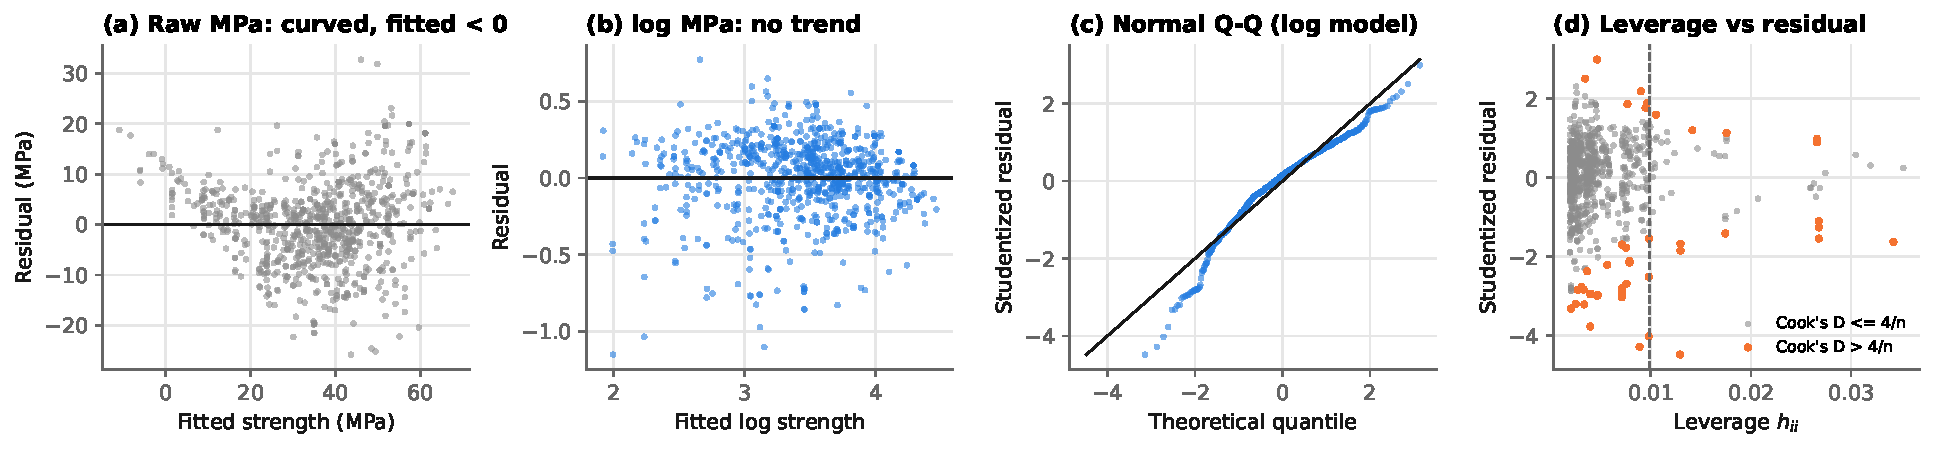
\includegraphics[width=\textwidth]{C1_diagnostics.pdf}
\caption{Diagnostics of model~\eqref{eq:law} with $d=2$ on training mixtures. (a) raw-scale residuals; (b)--(d) log scale: residuals vs fitted, normal Q--Q of studentized residuals, leverage $h_{ii}$ vs studentized residual (dashed: $2\bar h$; orange: Cook's $D_i>4/n$).}
\label{fig:diag}
\end{figure}

\paragraph{Q1: the law.} AIC keeps falling up to $d=\DAIC$, BIC is minimized at $d=\DBIC$, and grouped CV is flat in $d$: every degree lies within one standard error of the best, and the one-SE rule gives $d=\DCVse$ (Fig.~\ref{fig:sel}a). We adopt BIC's $d=\Dsel$, since extra age terms do not improve out-of-sample error. The fitted law has $\hat\beta_1=\BetaWB$ (SE \SeWB; 95\% CI $[\WBlo,\WBhi]$; $t=\TWB$) and $R^2=\LawRsq$. Strength therefore falls by \PctPerTenth\% for every 0.1 increase in $\wb$ ($\hat B=e^{-\hat\beta_1}=\AbramsB$). Abrams' original ratio $w/c$ explains less ($R^2=\LawWCRsq$). Because repeated tests of a mixture are correlated, the SE above is optimistic. Refitting on 28-day tests only, one per mixture ($n=\NTwentyEight$), gives $\hat\beta_1=\BetaWBtwentyEight$ (SE \SeWBtwentyEight), the same slope with an honest, larger SE. Fig.~\ref{fig:sel}b shows the fitted Abrams curves.

\begin{figure}[t]\centering
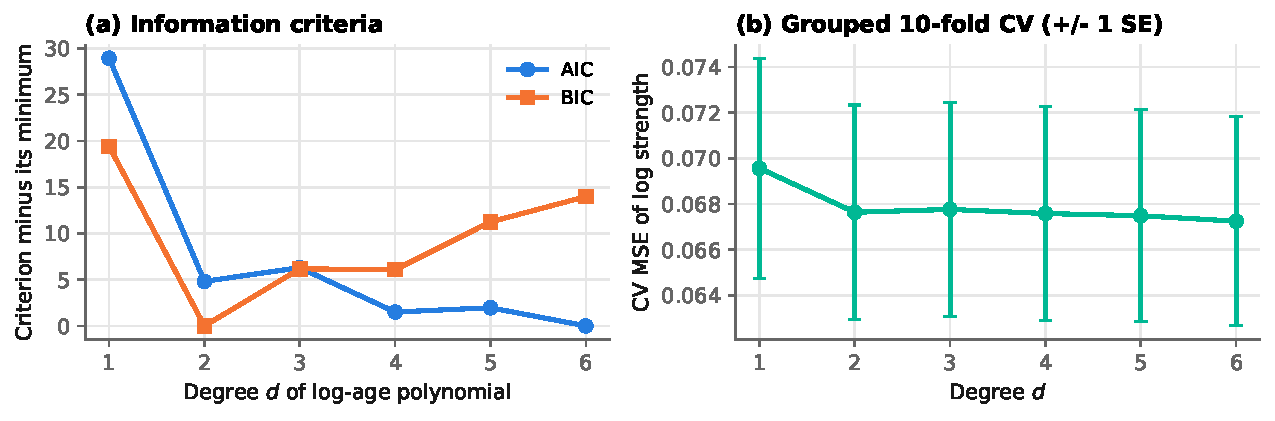
\includegraphics[width=0.53\textwidth]{C2_degree_selection.pdf}\hfill
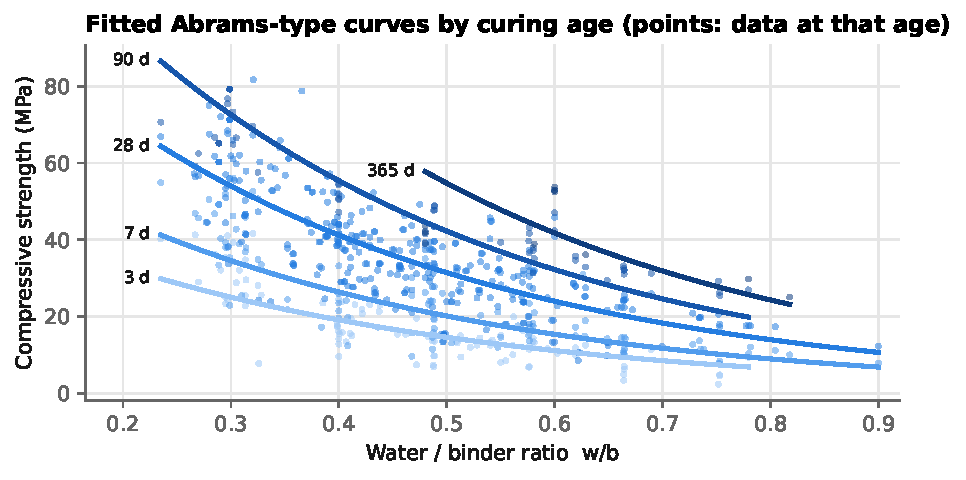
\includegraphics[width=0.45\textwidth]{C4_abrams_curves.pdf}
\caption{(a) Choosing the degree $d$ of the log-age polynomial: AIC and BIC relative to their minima, and grouped 10-fold CV MSE $\pm1$ SE. (b) Fitted law ($d=\Dsel$) by curing age, drawn only over the $\wb$ range observed at that age.}
\label{fig:sel}
\end{figure}

\paragraph{Q2: what the ingredients add.} Table~\ref{tab:comp} compares models on CV and on the \NMixTest{} held-out mixtures, where CV and test errors agree closely. The law with $\wb$ predicts held-out log strength with RMSE \TestWB{} (typical error \MapeWB\%). Adding the binder composition lowers this to \TestWBplus{} (\MapeWBplus\%), better than the seven raw amounts with the same ten coefficients (\TestIng). The physics-based parametrization therefore uses the information more efficiently. Its coefficients are interpretable. At 28 days, replacing 30\% of the cement with slag lowers strength by \ReplSlagTwentyEight\%, but the positive slag$\times a$ interaction ($\hat\beta=\BetaSlagAge$, $t=\TSlagAge$) turns this into \ReplSlagYear\% at one year. Fly ash costs \ReplAshTwentyEight\% at 28 days and still \ReplAshYear\% at one year ($t=\TAshAge$ for the interaction). This is the slow pozzolanic strength gain known to engineers, recovered from the data. Given $\wb$, superplasticizer adds nothing ($t=\TSP$), consistent with its role of letting mixes use less water. The 44-term quadratic model improves further to \TestQuadOLS{} (\MapeQuadOLS\%), so ingredient interactions carry some additional signal.

\begin{table}[t]\centering\small
\caption{Out-of-sample error of log strength. $p+1$: estimated coefficients. CV: grouped 10-fold on training mixtures. Test: \NMixTest{} held-out mixtures. MAPE: mean $|\hat f-f|/f$ on the test set.}
\label{tab:comp}
\begin{tabular}{lrrrrr}
\toprule
Model & $p+1$ & BIC & $\sqrt{\text{CV}}$ & Test RMSE & Test MAPE (\%)\\
\midrule
Abrams: $w/c$ + age ($d=\Dsel$) & \PWC & \BICWC & \CVWC & \TestWC & \MapeWC\\
Abrams: $\wb$ + age ($d=\Dsel$) & \PWB & \BICWB & \CVWB & \TestWB & \MapeWB\\
$\wb$ + binder composition + age & \PWBplus & \BICWBplus & \CVWBplus & \TestWBplus & \MapeWBplus\\
Seven raw amounts + age & \PIng & \BICIng & \CVIng & \TestIng & \MapeIng\\
Quadratic expansion, OLS & \PQuadOLS & \BICQuadOLS & \CVQuadOLS & \TestQuadOLS & \MapeQuadOLS\\
Quadratic, ridge ($\lambda_{\mathrm{CV}}$) & -- & -- & \CVRidge & \TestRidge & \MapeRidge\\
Quadratic, lasso ($\lambda_{\mathrm{CV}}$; \NZLasso{} nonzero) & -- & -- & \CVLasso & \TestLasso & \MapeLasso\\
Quadratic, lasso (1-SE; \NZLassoSE{} nonzero) & -- & -- & \CVLassoSE & \TestLassoSE & \MapeLassoSE\\
\bottomrule
\end{tabular}
\end{table}

\paragraph{Q3: regularization.} For the quadratic model, grouped CV error keeps falling as $\lambda$ decreases for both ridge and lasso, with its minimum at the smallest $\lambda$ on each grid (Fig.~\ref{fig:reg}b). The CV-optimal penalty is essentially zero, so neither improves on OLS. With $n=\NTrain$ against 44 features there is little variance to trade for bias. The one-SE lasso keeps \NZLassoSE{} of 44 terms with the same test error (\TestLassoSE), a sparser but equally accurate model. On a design that offers the lasso both raw amounts and ratios (Fig.~\ref{fig:reg}a), the first variables to enter as $\lambda$ decreases are \FirstEntry{} and \SecondEntry{}, followed by $w/c$. The raw ingredient amounts enter only later, with small coefficients. The lasso thus rediscovers the water--binder ratio. This is evidence about prediction, not causation, and correlated predictors make the entry order unstable (note the wiggles in the $\wb$ path).

\begin{figure}[t]\centering
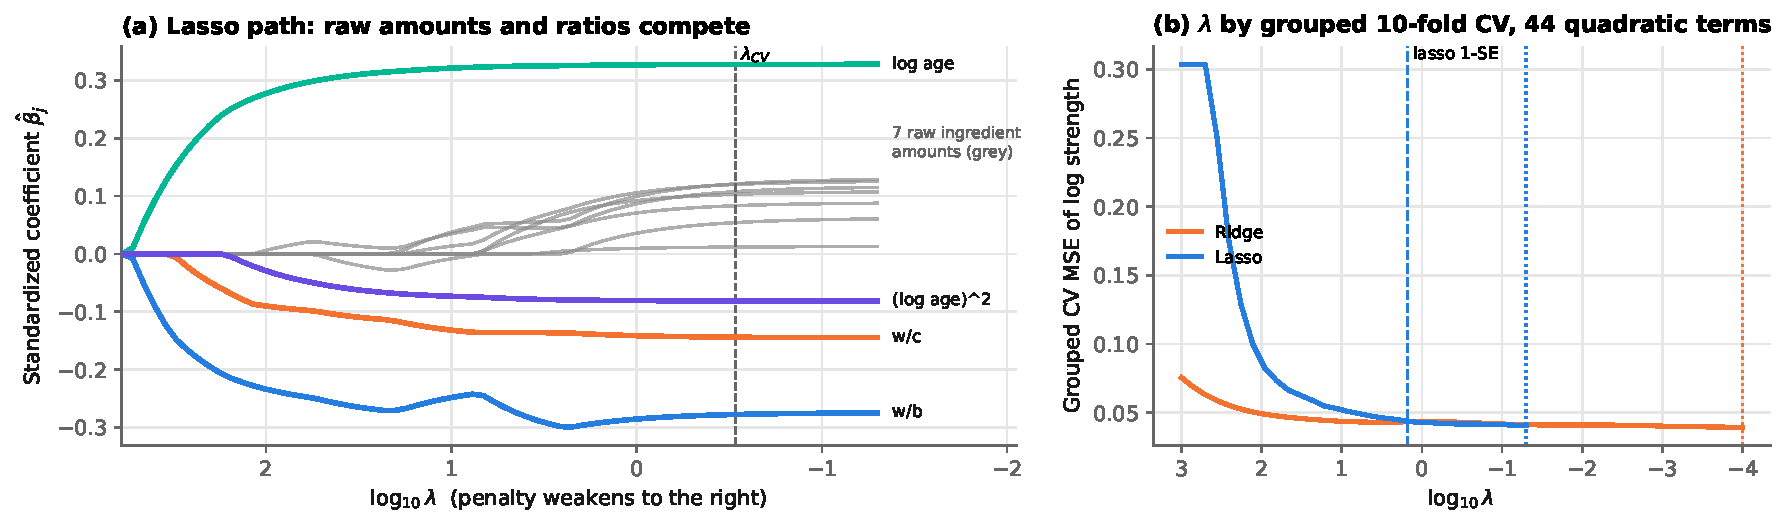
\includegraphics[width=\textwidth]{C3_regularization.pdf}
\caption{(a) Lasso path on standardized raw amounts, both ratios and log-age terms; dashed line: $\lambda$ chosen by grouped CV. (b) Grouped CV MSE for ridge and lasso on the 44-term quadratic expansion; dotted lines: CV minima; dashed: lasso one-SE choice.}
\label{fig:reg}
\end{figure}

\section{Interpretation and limitations}
A two-variable law from 1918 explains most of the variation in strength and predicts unseen mixtures to within about \MapeWB\%. Describing how the binder is composed closes \GapShare\% of the gap to the best model with ten coefficients instead of 45, and flexible models with or without shrinkage give only modest further gains. Several limits apply. (1) The data pool several laboratories \citep{yeh1998} whose curing and testing conditions are not recorded. Unexplained variation may partly be lab differences, and predictions apply to similar mixes only. (2) Coefficient SEs assume independent, constant-variance errors. Neither holds exactly (repeated mixtures; higher variance at early ages), so we rely on grouped CV and a held-out test set for model comparison, and on the 28-day subset for an honest SE of $\beta_1$. (3) Recipes were not randomized: the slag and fly-ash effects are associations conditional on $\wb$ and age, and may reflect other features of the mixes that used them. (4) Errors are computed on the log scale; back-transforming $\exp(\hat Y)$ estimates the median, not the mean, strength.

\paragraph{Reproducibility.} \texttt{python src/concrete\_analysis.py} regenerates every figure, the table and every number in this report (written to \texttt{macros.tex}); \texttt{python -m pytest} runs 31 unit tests.

\small
\begin{thebibliography}{9}
\bibitem[Abrams(1918)]{abrams1918} Abrams, D.~A. (1918). \emph{Design of Concrete Mixtures}. Bulletin~1, Structural Materials Research Laboratory, Lewis Institute, Chicago.
\bibitem[Hastie et~al.(2009)]{hastie2009} Hastie, T., Tibshirani, R., and Friedman, J. (2009). \emph{The Elements of Statistical Learning}, 2nd ed. Springer.
\bibitem[Maddu(2026)]{maddu2026} Maddu, S. (2026). \emph{Applied Statistics and Data Science I: Lecture Notes 12--16}. Johns Hopkins University.
\bibitem[Yeh(1998)]{yeh1998} Yeh, I.-C. (1998). Modeling of strength of high-performance concrete using artificial neural networks. \emph{Cement and Concrete Research}, 28(12), 1797--1808.
\bibitem[Yeh(2007)]{ucidata} Yeh, I.-C. (2007). Concrete Compressive Strength [Dataset]. UCI Machine Learning Repository. \url{https://doi.org/10.24432/C5PK67}.
\end{thebibliography}
\end{document}
